\documentclass[14pt]{extarticle}
\usepackage{fontspec}
\usepackage{polyglossia} % use instead of babel
\usepackage{pgfplots}
\usepackage{float}
\usepackage{amsmath}
\setdefaultlanguage{hebrew}
\setotherlanguage{english}
\newfontfamily\hebrewfont[Script=Hebrew]{Arial}

% TODO: figure out if better to keep this or not, for word document pdf output similarity
\usepackage[margin=1in]{geometry}

% might be useful to ensure similarity to word document pdf output
% \usepackage{setspace}
% \singlespacing

% Reset equation counter at the start of each section
\usepackage{chngcntr}
\usepackage{etoolbox}
\counterwithin*{equation}{section}
\preto{\section}{\setcounter{equation}{0}}

\begin{document}

\begin{center}
    {\LARGE \textbf{ממ"ן 13}}\\
    {\textbf{חוקי ניוטון}}
\end{center}

\begin{itemize}
    \item מגישים: תומר רוזנפלד, שי רואימי
    \item תאריך ביצוע הניסוי: 28 יולי 2025
    \item מדריך הניסוי: ד"ר סילביו ריינהורן
\end{itemize}
\newpage

\section*{ניסוי 1 - החוק הראשון של ניוטיון}
\subsection*{מטרת הניסוי}
בדיקת תוקפו של החוק הראשון של ניוטון
\subsection*{רקע תיאורטי}
החוק הראשון של ניוטון קובע כי גוף ששקול הכוחות עליו הוא אפס נשאר מתמיד במצב מנוחה או בתנועה במהירות קבועה בקו ישר.
\subsection*{מערכת המדידה ומהלך הניסוי}
ראשית איזנו מסילה כך שהייתה אופקית לחלוטין. בדקנו את אופקיות המסילה ע"י הנחת עגלה במקומות שונים על המסילה וראינו שהיא נשארה במקום.  בנוסף בדקנו בעזרת פלס.

בקצה של המסילה חיברנו חיישן תנועה, בניסוי זה  נעזרנו בו למדידת מיקום העגלה.

לאחר מכן דחפנו קלות את העגלה והקלטנו את תוצאות המדידה בתוכנת PASCO Capstone. המדידה הכילה את מיקום העגלה ביחס לזמן התחלת ההקלטה.

\subsection*{תוצאות וניתוח}
הגרף הבא מציג את מיקום העגלה ביחס לזמן: 
\begin{figure}[H]
    \centering
    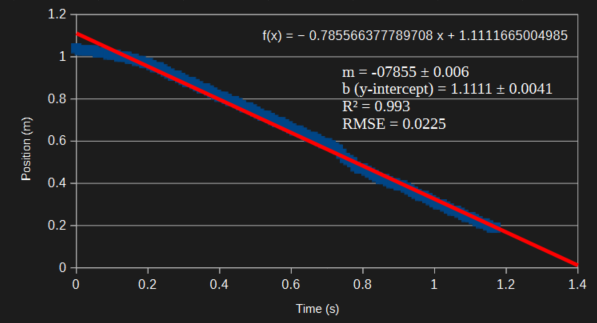
\includegraphics[width=0.8\textwidth]{maman_13_experiment_1_position_time_graph.png}
    \caption{מיקום העגלה ביחס לזמן}
\end{figure}

ניתן לראות שהגרף מתואר היטב ע"י פונקציה ליניארית עם שיפוע $m=0.7856$ ולכן:
\begin{center}
\begin{equation}
\begin{aligned}
    x(t) = x_0 + v_0 t + \frac{1}{2} a t^2 \\
    x_0 = 1.1111 \\
    a = 0 \\
    v_0 = \textbf{שיפוע הגרף} = -0.7856 \\
\end{aligned}
\end{equation}
\end{center}
סימן המינוס הוא מכיוון שכיוון התנועה של העגלה הוא לכיוון חיישן התנועה.

\subsection{דיון ומסקנות}
בניסוי שקול הכוחות על הגוף בציר התנועה (המסילה) היה אפס וכך יכלננו לבדוק את קיום החוק הראשון של ניוטון.

במדידה קיבלנו גרף מקום ביחס לזמן, עם התאמה טובה לפונקציה ליניארית,  ומשם הסקנו כי מהירות הגוף קבועה - כלומר הגוף מתמיד במצב תנועה במהירות קבועה בקו ישר, כפי שקובע החוק הראשון של ניוטון.

החוסר התאמה הליניארית בגרף יכולה לנבוע מחיכוך, כאשר החיכוך עלול להשתנות גם כתלות במיקום הגוף על המסילה (המסילה אינה חלקה לכל אורכה), וגם אולי משיפוע קל במסילה.


\end{document}